%************************************************
\chapter{Aprendizaje automático}\label{ch:ML}
% ************************************************
%--- Deep Learning Ian G book
% Historical dev
% big data &  improve of memorie in computer
% poner el puto diagramita q siempre sale

%\begin{flushright}{\slshape
 %   El aprendizaje automático es como una caja de bombones: nunca sabes lo que vas a obtener... a menos que tengas buenos datos y una sólida comprensión de tus algoritmos.} \\ \medskip
  %  --- ChatGPT AI language model
%\end{flushright}



La \textbf{inteligencia artificial}, o AI por sus siglas en inglés, se puede definir como un sistema capaz de interactuar con su entorno. Algunos ejemplos de inteligencias artificiales son: \emph{Siri} de Apple y \emph{Alexa} de Amazon. Para poder generar una respuesta al entorno, estos sistemas contienen sensores que permiten la entrada de información, en estos ejemplos la información es obtenida mediante la voz o las palabras escritas de los usuarios, esta información es procesada a través de métodos de aprendizaje automático o ML por sus siglas en inglés.

\begin{figure}[!htbp]
  \centering
  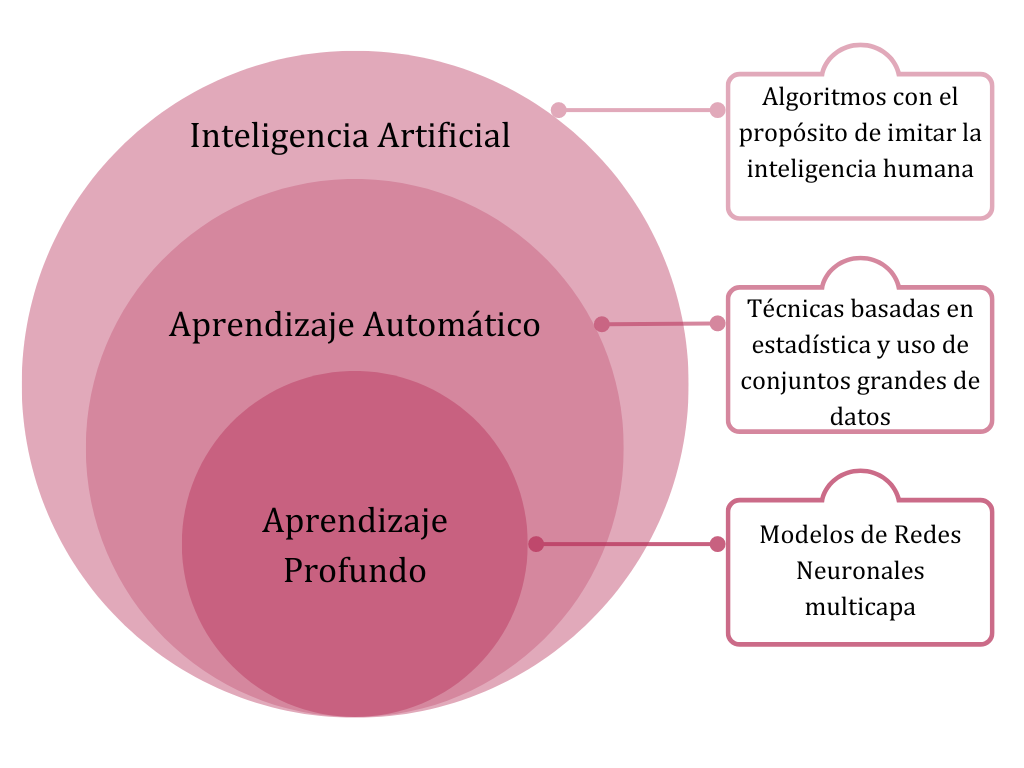
\includegraphics[width=0.7\textwidth]{./img/IA_ML_DL.png}
  \caption{Diagrama de Venn que muestra los conceptos de inteligencia artificial, aprendizaje automático y aprendizaje profundo.}
  \label{fig:IA-ML-DL}
\end{figure}

Los métodos de \textbf{aprendizaje automático} se pueden definir como un conjunto de métodos que pueden detectar automáticamente patrones en datos y aplicarlos para predecir nuevos datos. A grandes rasgos, los métodos de aprendizaje automático pueden dividirse en dos categorías: aprendizaje supervisado y aprendizaje no supervisado \cite{murphy:2013}.

\section{Aprendizaje supervisado}
En el \textbf{aprendizaje supervisado} el objetivo es aprender a partir de un conjunto de $M$ datos de entrenamiento definidos como:
\begin{equation}
\{\vec{x}_i, y_i\}_{i=1}^{M},
\end{equation}
una forma de mapear $\vec{x}_i$ a $y_i$.
\\
Cada vector:
\begin{equation}
  \label{eq:trainset}
\vec{x}_i = (x_1,x_2, \dots , x_d)_i,
\end{equation}
corresponde a un dato, en donde cada componente es una \textbf{característica} o \textbf{atributo} del dato en cuestión, y el número de componentes depende del problema. Algunos ejemplos de $\vec{x}_i$ son:
\begin{itemize}[label=\textcolor{CTtitle}{\textbullet}]
\item Imágenes
\item Enunciados de texto
\item Audios de voz
\item Series de tiempo
\end{itemize}

Por otro lado, $y_i$ corresponde a la \textbf{etiqueta} de $\vec{x}_i$. Si $y_i$ toma un valor categórico, es decir, pertenece a un conjunto finito de categorías:
$$y_i \in \{1,\dots,c\}, \text{  por ejemplo: 1=perro, 2=gato, etc. }$$ 
se dice que el problema es de \textbf{clasificación}.
En cambio, si $y_i$\footnote{$y_i$ puede ser también un vector $\vec{y}_i$, en donde su dimensión está determinada por el problema a resolver, y no necesariamente es igual a la de $\vec{x}_i$.} es un valor real, se dice que el problema es de \textbf{regresión}.
\\

Algunos ejemplos de métodos de aprendizaje supervisado son:
\begin{itemize}[label=\textcolor{CTtitle}{\textbullet}]
\item Árboles de desición: Para problemas de clasificación
\item Regresión lineal: Para problemas de regresión
\item Redes Neuronales: Para problemas de regresión y de clasificación
\end{itemize}

\section{Aprendizaje no supervisado}
En el \textbf{aprendizaje no supervisado} el conjunto de entrenamiento de $M$ datos se reduce a:
\[ \{\vec{x}_i\}_{i=1}^M \]
en donde no se cuenta con una etiqueta $y_i$. En este tipo de problemas, los métodos están enfocados en buscar patrones importantes a partir de únicamente los datos de entrada.
\\
Algunos ejemplos de métodos de aprendizaje no supervisado son:
\begin{itemize}[label=\textcolor{CTtitle}{\textbullet}]
\item Clustering: Agrupar datos similares entre sí
\item Análisis de Componentes Principales: Buscar la relación entre las característica de los datos y reducir su dimensionalidad
\end{itemize}

El \textbf{aprendizaje por refuerzo} es comúnmente considerado una tercer categoría de aprendizaje automático, de manera general, en estas técnicas el sistema inteligente interactúa con su entorno con el objetivo de obtener recompensas, bajo el contexto en el que se está implementando, a menudo se utiliza este tipo de aprendizaje para enseñar a las máquinas cómo jugar video juegos \cite{Ivan:2019}.

\section{Aprendizaje profundo}
El \textbf{aprendizaje profundo}, o \textbf{deep learning} \cite{Bengio2009} en inglés, como se muestra en la \autoref{fig:IA-ML-DL}, es un sub-campo del aprendizaje automático, que puede definirse como aquellos métodos que procesan la información en múltiples capas, en donde el nivel de abstracción y complejidad de la información incrementa conforme avanza de una capa a la siguiente.
\\
En la práctica, los modelos de aprendizaje profundo son redes neuronales artificiales multicapa (\autoref{ch:NNBasics}). Algunos ejemplos comúnmente utilizados son \cite{Ivan:2019}:
\begin{itemize}[label=\textcolor{CTtitle}{\textbullet}]
\item Perceptrones Multicapa \autoref{sec:multicapamodels}
\item Redes Neuronales Convolucionales
\item Redes Neuronales Recurrentes \autoref{sec:RNN}
\end{itemize}

En el siguiente capítulo se abordarán conceptos básicos acerca de las redes neuronales artificiales, cómo están construidas, es decir, su arquitectura; y cómo, de manera general, este tipo de algoritmos aprenden con base al procesamiento de múltiples datos o muestras de ejemplo.



